\documentclass{standalone}
\usepackage{tikz}
\usetikzlibrary{positioning, circuits.ee.IEC, arrows, decorations.pathreplacing}

\begin{document}
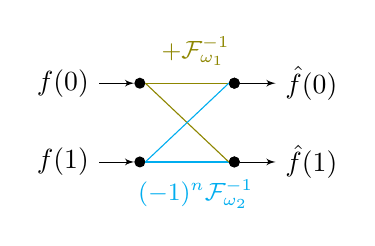
\begin{tikzpicture}
[
    yscale=1.0, xscale=1.2, node distance=0.3cm, auto,
    % The strategy is to create nodes with names: N-column-row
    % Input nodes are named N-0-0 ... N-0-7
    % Output nodes are named N-8-0 ... N-8-5
    circuit ee IEC
]

%=================================== Start ===================================
\tikzstyle{n}   = [circle, fill, minimum size=4pt,inner sep=0pt, outer sep=0pt]
\tikzstyle{mul} = [circle, draw, inner sep=-1pt]
\tikzstyle{box} = [
    draw, align=center, shape=rectangle, minimum width=1.5cm, minimum height=3.5cm,
    append after command={
        % see also: https://tex.stackexchange.com/a/129668
        \foreach \side in {east, west} {
            \foreach \i in {1,...,#1} {
            %  oordinate (\tikzlastnode-\i-\side)
            %  at ($(\tikzlastnode.north \side)!{(\i-.5)/(#1)}!(\tikzlastnode.south \side)$)
                (\tikzlastnode.north \side) edge[draw=none, line to]
                    coordinate[pos=(\i-.5)/(#1)] (\tikzlastnode-\i-\side) (\tikzlastnode.south \side)
            }
        }
    }
]

% Define two helper counters
\newcounter{x} \newcounter{y}
{
    % \node[box=4] (box-t) {$N = \frac{T}{2}$ \\\\ DFT};
    % \node[box=4, below=of box-t] (box-b) {$N = \frac{T}{2}$ \\\\ DFT};

    % Draw inputs
    \foreach \y in {0,...,1}
        \node[n, pin={[pin edge={latex'-,black}]left:$f(\y)$}]
              (N-0-\y) at (0,-\y) {};
    % Draw outputs
    \foreach \y / \idx in {0/0, 1/1}
        \node[n, pin={[pin edge={-latex',black}]right:$\hat{f}(\idx)$}]
              (N-2-\y) at (1,-\y) {};
   % draw connector nodes
    \foreach \y in {0,...,1}
        \foreach \x / \c in {1/1}
            \node[n, name=N-\c-\y] at (\x,-\y) {};
   
    % horizontal connections
    % Note the use of simple counter arithmetics to get correct
    % indexes.
  
    \path (N-0-0) edge[-,olive] (N-1-0);
    \path (N-0-1) edge[-,cyan ] (N-1-1);
  
    % Connect nodes
    \foreach \sourcey / \desty in {0/1}
        \path (N-0-\sourcey.east) edge[-,olive] node[right = 17pt, above = 17pt] 
                {\small $\ \ +{\mathcal {F}}_{\omega_1}^{-1}$} 
              (N-2-\desty.west);
    \foreach \sourcey / \desty in {1/0}
        \path (N-0-\sourcey.east) edge[-,cyan ] node[right = 17pt, below = 17pt] 
                {\small $\ \ (-1)^n {\mathcal {F}}_{\omega_2}^{-1}$} 
              (N-2-\desty.west);
}
%==================================== END ====================================

\end{tikzpicture}
\end{document}